% !TeX spellcheck = en_GB
\chapter{Results and Discussion}\label{kap:results}
\section{Effect of Gene Conversion on the GFS}
The effect of gene conversion on the gene frequency spectrum becomes most apparent when simulations are performed on a fixed tree with a recognisable \ac{GFS} pattern.
In our constructed tree (figure \ref{fig:tree-gc-loss}) with three distinct clades (C1: individuals 0-3, C2: individuals 4-7, C3: individuals 8-9),
the two leftmost clades consist of four individuals each, while the right clade consists of only two.
Due to numerous gene gain events along the long branch from node 18 to 17, we expect these genes to spread across the entire left side, resulting in a \ac{GFS} peak at class 8.
Similarly, along the branches 17 to 15 and 17 to 16, the gene gain affects the entire clade, resulting in a \ac{GFS} peak at class 4.
The same principle applies to the 18 to 14 branch, but for the smaller clade, resulting in a peak at class 2.
Genes present in all 10 individuals are less likely to stem from regular event as this would require at least two gene gain events at the same site on different branches, but rather stem from the ancestral state.
As the \ac{GFS} includes those and does not distinguish between those genes we expect another peak at class 10.
While it is easy to infer the GFS from a tree structure, it is not possible to do the inverse.


The introduction of a single gene conversion event causes a gene in a few individuals to follow an alternative phylogenetic tree.
This is illustrated by the light green segment / branches in the figure that oppose to the dominant tree in dark blue.
Due to the long edge from 18 top GC1 an increase of the peak Gene Frequency Class 6 would be expected.


As gene conversion increases, more genome segments are determined by different trees, disrupting the effect of the initial structure.
Consequently, the expected \ac{GFS} across different fixed trees with gene conversion converges towards the expected \ac{GFS} of random trees under neutral evolution.
Nevertheless, certain features persist even with increased gene conversion rates, such as the peak at class 4 and class 10.
These would require numerous gene conversion events to counteract the strong influence of long edges and the root probability of the ancestral state.
This is visible in figure \ref{fig:tree-gc-loss} (right) which depict the \ac{GFS} for different gene conversion rates and the mean $\chi^2$-like error.

\begin{figure}[h]
    \centering
    \begin{minipage}{0.49\textwidth}
        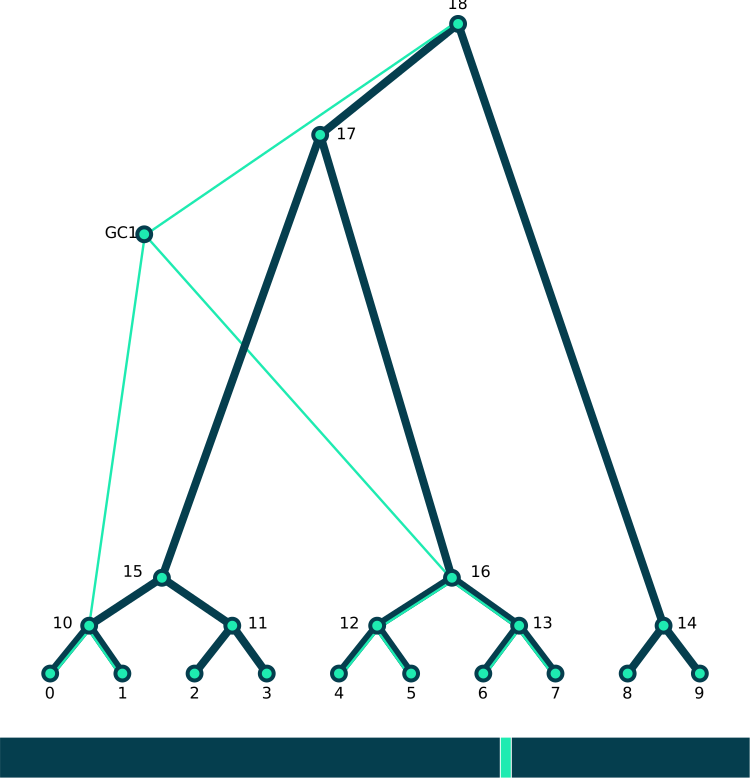
\includegraphics[width=\textwidth]{figures/effect_on_gfs/tree_with_gc.pdf}
    \end{minipage}
    \begin{minipage}{0.49\textwidth}
        \hfill\includegraphics[width=0.99\textwidth]{figures/effect_on_gfs/gfs_gc.pdf}\\
        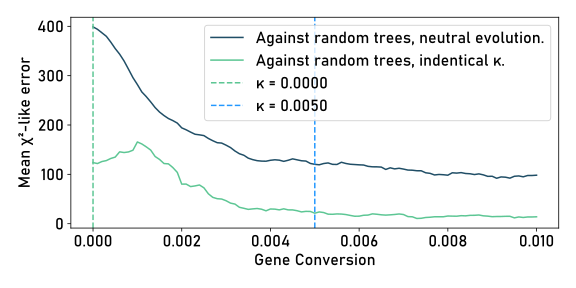
\includegraphics[width=\textwidth]{figures/effect_on_gfs/gfs_gc_factor.pdf}
    \end{minipage}
    \caption[Effect of gene conversion on the GFS.]{Tree with one gene conversion event (left), its GFS for different gene conversion rates (top right) and
        its respective $\chi^2$-like error (bottom right).}
    \label{fig:tree-gc-loss}
\end{figure}

When inspecting the non-normalized \ac{GFS} of simulations with a fixed tree, it apparently it does not exactly match the expected \ac{GFS} of neutral random trees.
Instead, it reflects its shape but is slightly shifted based on the gene gain/loss parameters.
This shift is caused by the emergence of new lineages due to gene conversion, which increases the time to coalescence for all lineages.
As a result, the total potential for gene gain / loss events is increased.
The $\chi^2$-like error between the mean \ac{GFS} and the expected \ac{GFS} highlights this discrepancy.
Initially, the error drops to a low level but never reaches zero.

\section{Effect of HGT on the GFS}
\begin{figure}[h]
    \centering
    \includegraphics[width=0.49\textwidth]{figures/effect_on_gfs/gfs_hgt.pdf}
    \includegraphics[width=0.49\textwidth]{figures/effect_on_gfs/gfs_hgt_levels_2.pdf}
    \caption[Effect of HGT on the GFS.]{GFS for different HGT rates (left) on a fixed tree and on random trees (right).}
    \label{fig:hgt-loss}
\end{figure}

A high value of $\gamma$ shifts the gene frequency spectrum to the right, indicating that most genes are present at high frequency resulting in a characteristic \reflectbox{L} shape.
This means that when new individuals are sequenced, it is unlikely that new genes will be discovered that were not previously observed.
When a fixed tree is used, a similar effect to gene conversion is expected.
Along with the loss of characteristic features of the simulated tree, a shift to the right is expected, resulting in a smaller peak at lower gene frequency classes.
This is due to new edges introduced by horizontal gene transfer events changing the original tree structure.
This effect is visible in figure \ref{fig:hgt-loss}.

The increase in gene frequency is due to the nature of \ac{HGT}, where any gene acquisition in a lineage, whether by vertical inheritance or \ac{HGT}, is counted as a gain.
This effect is clearly visible in figure \ref{fig:hgt-loss} for simulations without tree fixation.

\section{Neutrality test robustness}
The properties of the neutrality test differ between the $\chi^2$ approach and the direct approach.
Understanding these differences helps to interpret test results and to determine the situations in which each approach may be most informative.

By relying on the minimum p-value across all \ac{GFS} classes, the direct approach is sensitive to small changes within individual classes.
Small variations in the underlying parameters ($\theta, \rho, \gamma$ and $\kappa$) can lead to pronounced changes, especially at the edges of the \ac{GFS} in classes $1$ and $n$.
The direct approach also shows reduced sensitivity to overall upward or downward shifts in the GFS, as these large changes may not significantly alter individual class probabilities.
These changes are captured by the $\chi^2$ approach by summing the respective errors.

\subsection{With neutral evolution as reference}
We assessed the robustness of our model by calculating the mean likelihood values and 90\% percentiles obtained from multiple neutrality tests.
This provides a measure of the stability of the test under different assumptions about evolution.
A reference distribution was generated by sampling the \ac{GFS} of 5000 simulations under neutral parameters.
Then 25 simulations were run for each step in our list of desired parameters (table \ref{app:robust-param}, figure \ref{fig:robust_gc0}).

The plots of these results include a vertical blue line indicating the true parameters used in the neutral reference simulation:

\begin{itemize}
    \item \textbf{Gene Gain} ($\theta$): Tests around theta perform consistently well, forming the expected bell curve around the true parameter values.
          Deviations as large as 1000 lead to significant drops in p-values (below 0.1).
    \item \textbf{Gene Loss} ($\rho$): A similar pattern can be observed for Rho. Here we see a saturation effect, as at high gene loss values the effect is less pronounced,
          as most events occur at sites where no gene is already present.
    \item \textbf{Gene Conversion} ($\kappa$): As higher gene conversion rates shift the gene frequency spectrum towards that expected from random tree models, the variance of the \ac{GFS} decreases.
          As a result, the tests do not detect deviations due to increased gene conversion rates.
          However, if a simulation with gene conversion ($\kappa$ = 2) is used as a reference, it is possible to detect values originating from a simulation with low gene conversion.
    \item \textbf{HGT} ($\gamma$): The effect of \ac{HGT} is clearly visible, with a half bell curve around the true value.
          As the effect of \ac{HGT} is strong on individual GF classes as well as all classes together, it is well picked up by the $\chi^2$ based and direct test
\end{itemize}
\begin{figure}[]
    \centering
    \begin{minipage}{0.49\textwidth}
        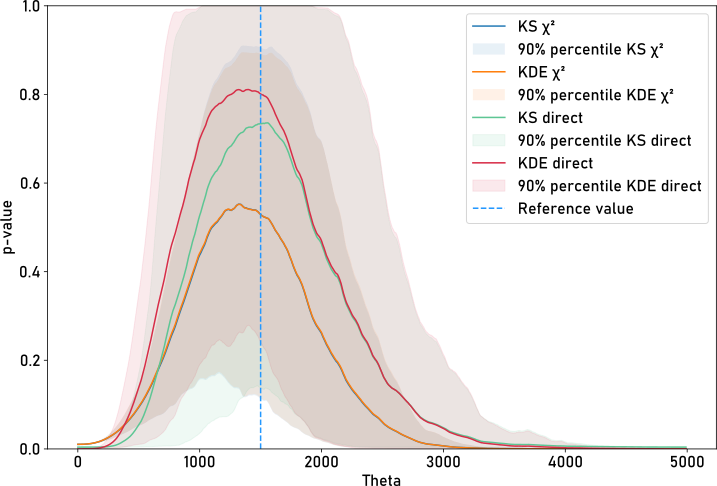
\includegraphics[width=\textwidth]{figures/neutrality_test/gc_0_theta.pdf}\\
        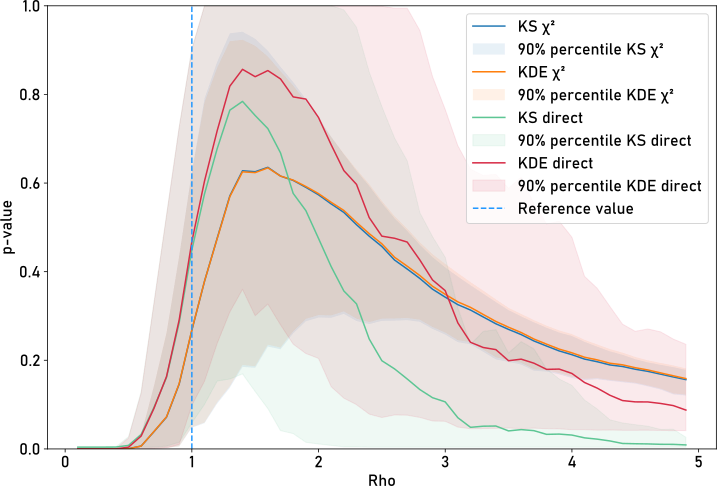
\includegraphics[width=\textwidth]{figures/neutrality_test/gc_0_rho.pdf}
    \end{minipage}
    \begin{minipage}{0.49\textwidth}
        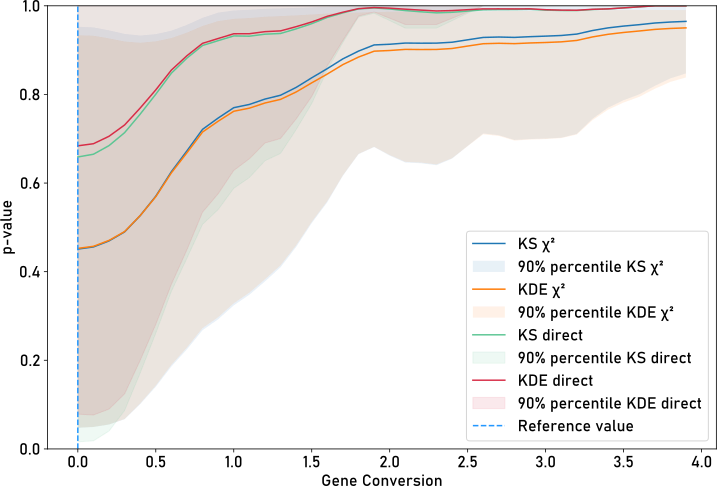
\includegraphics[width=\textwidth]{figures/neutrality_test/gc_0_gc.pdf}\\
        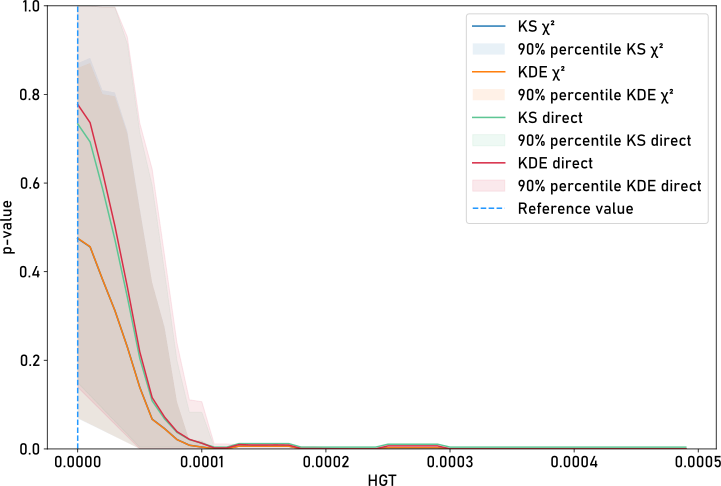
\includegraphics[width=\textwidth]{figures/neutrality_test/gc_0_hgt.pdf}
    \end{minipage}
    \caption[Robustness of the neutrality test for $\kappa = 0$.]{Robustness of the neutrality test for different $\theta$ (top left), $\rho$ (bottom left), $\kappa$ (top right), $\gamma$ (bottom right) values
        with a neutral evolution as reference.}
    \label{fig:robust_gc0}
\end{figure}

\subsection{Non-neutral evolution as reference}

As the neutrality test is based on a simulated reference distribution it is also possible to test against an evolution with gene conversion or \ac{HGT}.
When considering non-neutral evolutionary processes, the expected gene frequency spectrum distribution must be adjusted accordingly.
In the following test, the reference distribution was obtained by simulating with $\gamma = 0.0001$.
A total of 5000 samples were recorded.
Similar characteristics are observed for changes in $\theta$ and $\rho$: a bell curve around the true $\theta$ value and a tail for $\rho$ due to the saturation effect.
See figure \ref{fig:robust_hgt}.
The difference between the \ac{KDE}-smoothed and \ac{KS}-based $\chi^2$ test appears to be due to rare outliers.
These outliers affect the smoothing process, resulting in a wider distribution and therefore a less effective test.
For \ac{HGT}, the test is able to distinguish whether the new data stems from a simulation with less or no \ac{HGT}, and shows a right tailed bell curve.
This left part of the curve reflects the test results from the neutral evolution, as it is the inverted version if it.
For higher \ac{HGT} values, the sensitivity decreases and significantly higher \ac{HGT} values are required.
The reason for this is that the reference \ac{HGT} value of 0.0001 already has a strong effect on the gene frequency spectrum,
and the relative change for higher values is small as the effect saturates.
A similar pattern was observed for simulations with gene conversion ($\kappa = 2$, figure \ref{fig:robust_hgt} bottom right) as a reference.
Here the test is able to detect \ac{GFS} from the simulation with less gene conversion.
Detection of higher values of $\kappa$ is not possible, as the effect of gene conversion saturates after pushing the \ac{GFS} to the expected \ac{GFS} for random trees.

The complete list of measurement can be found in appendix \ref{app:robust_gc}.

\begin{figure}[h]
    \centering
    \begin{minipage}{0.49\textwidth}
        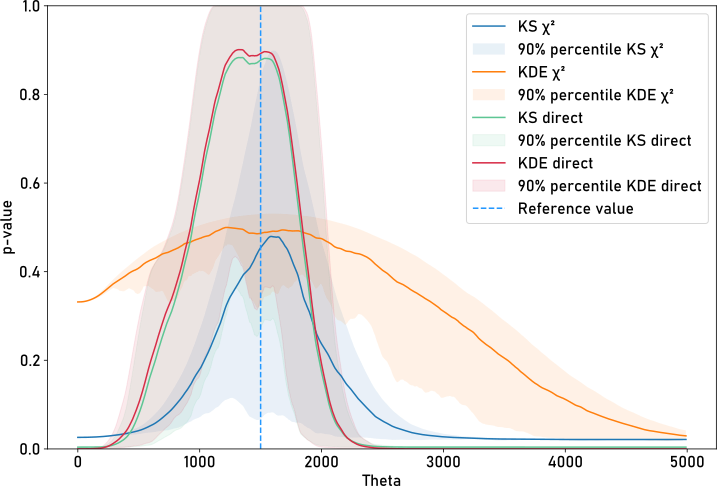
\includegraphics[width=\textwidth]{figures/neutrality_test/hgt_0.0001_theta.pdf}\\
        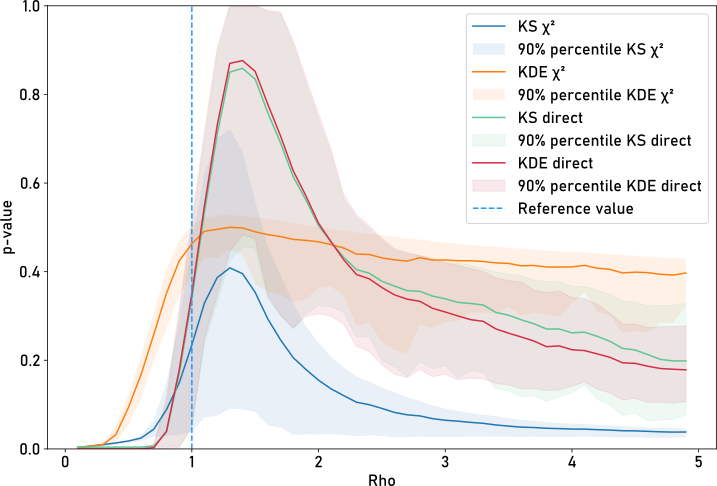
\includegraphics[width=\textwidth]{figures/neutrality_test/hgt_0.0001_rho.pdf}
    \end{minipage}
    \begin{minipage}{0.49\textwidth}
        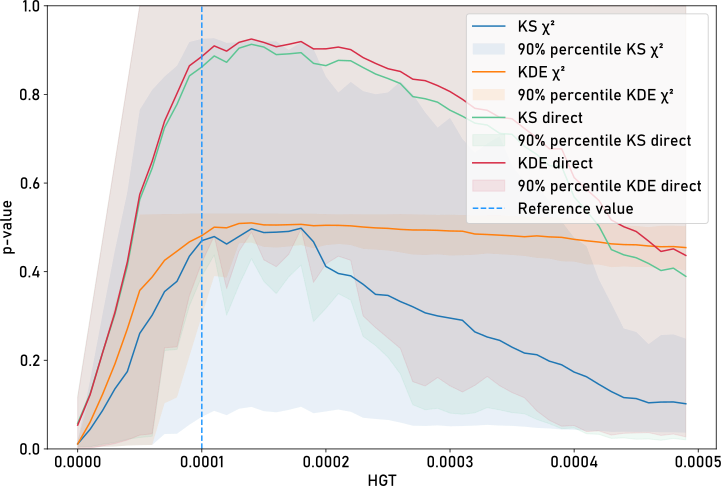
\includegraphics[width=\textwidth]{figures/neutrality_test/hgt_0.0001_hgt.pdf}\\ %hgt
        \includegraphics[width=\textwidth]{figures/neutrality_test/gc_2_gc.pdf} %gc2
    \end{minipage}
    \caption[Robustness of the neutrality test for $\gamma = 0.001$ and $\kappa = 2$ as reference.]{Robustness of the neutrality test for different $\theta$ (top left), $\rho$ (bottom left), $\kappa$ (top right), $\gamma$ (bottom right) values
        with $\gamma = 0.001$ (top / bottom left, top right) and $\kappa = 2$ (bottom right) as reference.}
    \label{fig:robust_hgt}
\end{figure}


\section{Runtime}
To ensure that the new gene model has a feasible runtime - necessary due to the multiple runs required for neutrality estimation - we investigated the effect of different parameters.

Simulations without \ac{HGT} are using the underlying C implementation, while those with \ac{HGT} are using a pure Python implementation.
This difference is expected to lead to significant differences in runtime.
To capture this effect, we timed a wide range of values for the parameters $n$, $s$, $\theta$, $\rho$ and $\kappa$ with a \ac{HGT} rate $\gamma$ set to 0 and 0.001.
Each parameter was tested in isolation, i.e. only one parameter was varied while the others were held constant at their default settings.

The parameters, their default values and their ranges tested were as follows:
\begin{table}[h]
    \begin{adjustbox}{width=\textwidth}
        \begin{tabular}{r|lllll}
            Parameter & Min  & Max    & Step   & Default    & Description                    \\
            \hline
            $n$       & 0    & 10000  & 10     & 10         & Number of samples.             \\
            $s$       & 1000 & 100000 & 100    & 10000      & Number of sites.               \\
            $\theta$  & 0    & 1000   & 1      & 100        & Gene gain rate.                \\
            $\rho$    & 0.01 & 0.5    & 0.001  & 0.1        & Gene loss rate.                \\
            $\kappa$  & 0    & 2      & 0.01   & 0          & Gene conversion rate.          \\
            \hline
            $\gamma$  & 0    & 0.005  & 0.0005 & 0 / 0.0001 & Horizontal Gene Transfer rate.
        \end{tabular}
    \end{adjustbox}
    \caption{Runtime analysis parameters.}
\end{table}

A total of 100 simulations were run for each step within a parameter's range, and run times were recorded.
Some parameter combinations were also tested to identify potential pairwise dependencies.
The individual plots (figure \ref{fig:runtime}) show the mean runtimes and the 90th percentiles.
Figures presenting the remaining parameters, simulation with HGT and the first difference of the runtimes are shown in the appendix \ref{app:runtime}.
As inferred from the implementation, the runtime follows a mostly linear dependence on problem and parameter size.

\begin{itemize}
    \item \textbf{Number of samples}: Runtime anomalies were observed for certain sample sizes, particularly around 500 for the C implementation.
          Initial hypotheses suggested that these anomalies might be due to default memory allocations or processor cache limitations.
          However, tests on different processors, regardless of L2/L3 cache size, showed similar increases at these sample sizes.
          Thermal throttling or switching from performance to efficiency cores was considered but ruled out due to the consistent runtime jumps at these specific points.
          Given the small impact of these anomalies and their absence in the Python version, they were ignored for the remainder of the study.

    \item \textbf{Number of genes}: The graphs show an almost linear increase in runtime as the number of genes increases, with the difference showing a slightly super-linear trend.
          With more genes, more positions have to be tracked, causing the increase.

    \item \textbf{Gene Gain} ($\theta$): Both graphs and their derivatives show a stable linear growth in runtime with increasing theta, reflecting the additional computational load of more gene gain events and the resulting increase in the number of lines to track.

    \item \textbf{Gene Loss} ($\rho$): A lower rho value means fewer gene loss events, resulting in more lines to simulate. As rho increases, fewer lines need to be simulated due to more frequent gene losses.
          However, at a certain point, simulating gene loss events takes longer than the time saved by eliminating lines, leading to a linear increase in run time.
          To fully understand the interaction between rho and theta, we plotted the execution time over a range of their combinations and ratios.

    \item \textbf{Ratio of $\rho$ to $\theta$}: The runtime for different ratios of $\theta$ and $\rho$ is presented in figure \ref{app:theta-rho-heatmap}.
          The effect of $\rho$ on runtime initially decreases execution time, followed by a linear increase as $\rho$ increases.
          In this analysis, the parameter range was set from 0 to 10,000 in steps of 100 for $\theta$ and 0 to 1 in steps of 0.01 for $\rho$.
          All possible combinations were measured, and the parameter grid was shuffled to reduce the impact of sorting bias.
          Outliers in the heatmap are likely due to measurement methods, as there is no clear pattern.\\
          \newpage
    \item \textbf{Gene Conversion} ($\kappa$): This parameter has a significant effect on running time, with a more than linear increase observed.
          Each gene conversion event introduces a new lineage into the population, increasing the number of generations required to reach the most recent common ancestor.

    \item \textbf{HGT} ($\gamma$): Similarly to gene conversion, this parameter has a strong effect on run time. Each \ac{HGT} event creates a new lineage that must be tracked and post-processed, leading to a superlinear increase in runtime.
\end{itemize}

Overall, these results highlight the impact of the number of lineages on the runtime and the need for a C implementation.
\begin{figure}[H]
    \begin{flushright}
        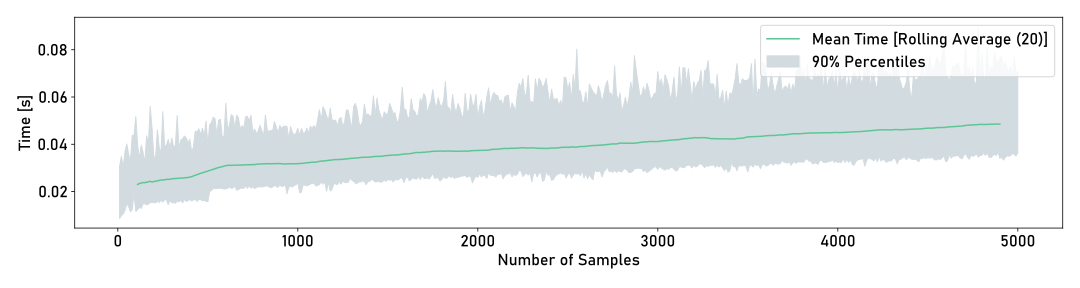
\includegraphics[width=\textwidth]{figures/runtime/num_samples.pdf}\\
        \includegraphics[width=\textwidth]{figures/runtime/num_sites.pdf}\\
        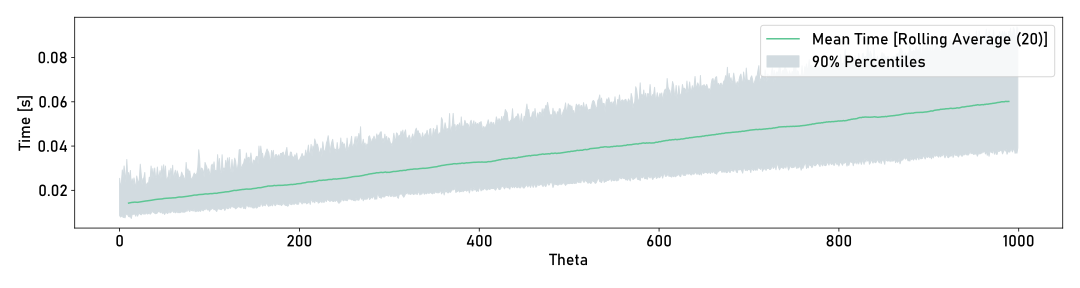
\includegraphics[width=\textwidth]{figures/runtime/theta.pdf}\\
        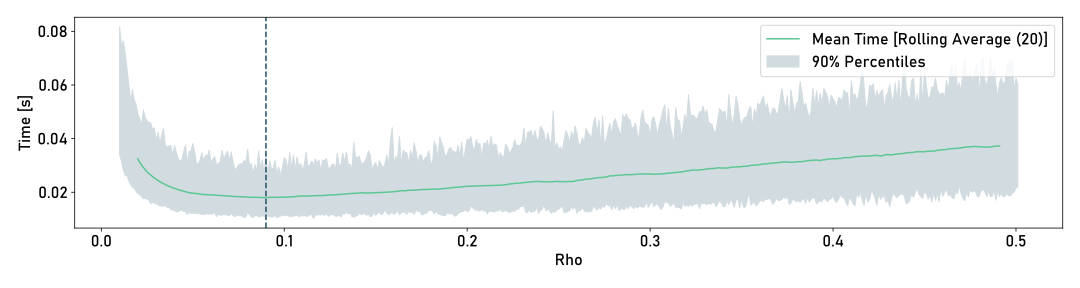
\includegraphics[width=\textwidth]{figures/runtime/rho.pdf}\\
    \end{flushright}
    \centering
    \caption[Runtime without HGT.]{Runtime of \mintinline{python}{gene_model} for different number of samples, number of sites, $\theta$ and $\rho$ rates
        for simulations without HGT.}
    \label{fig:runtime}
\end{figure}

\section{Estimating parameters for real world pangenomes}
\begin{figure}[H]
    \centering
    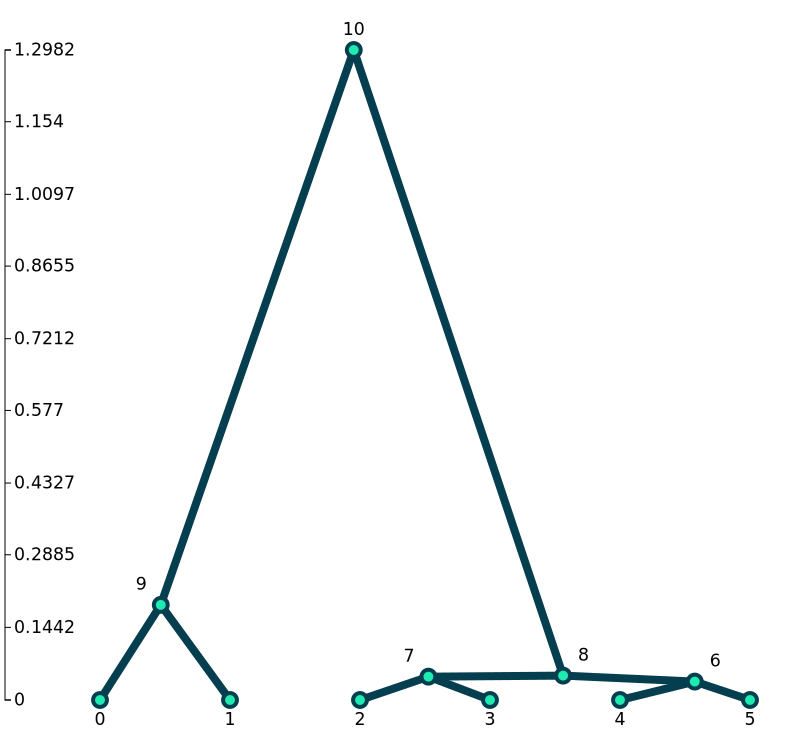
\includegraphics[width=0.49\textwidth]{figures/fitted_gfs/803.pdf}
    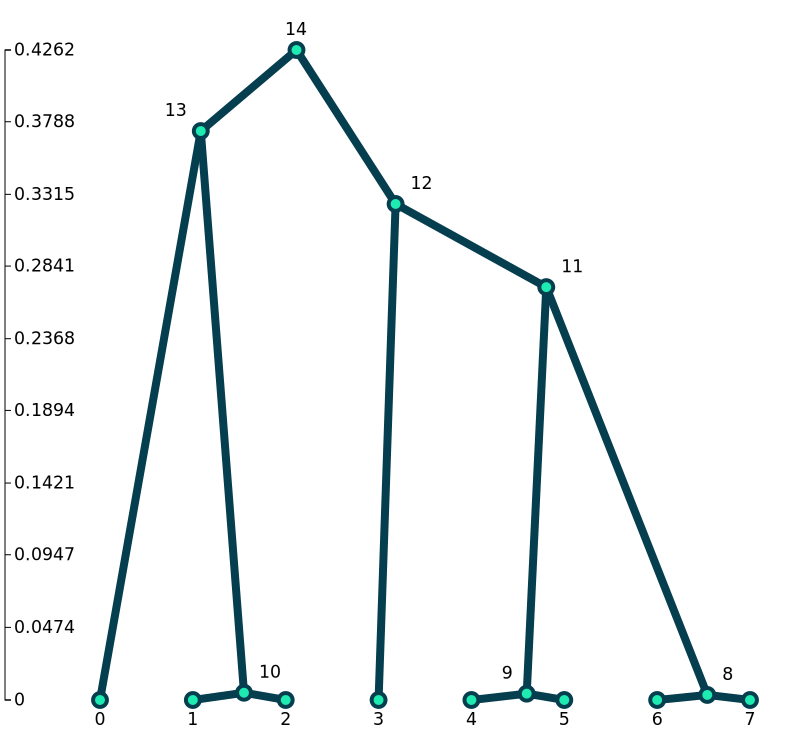
\includegraphics[width=0.49\textwidth]{figures/fitted_gfs/985002.pdf}\\
    \includegraphics[width=0.49\textwidth]{figures/fitted_gfs/1492.pdf}
    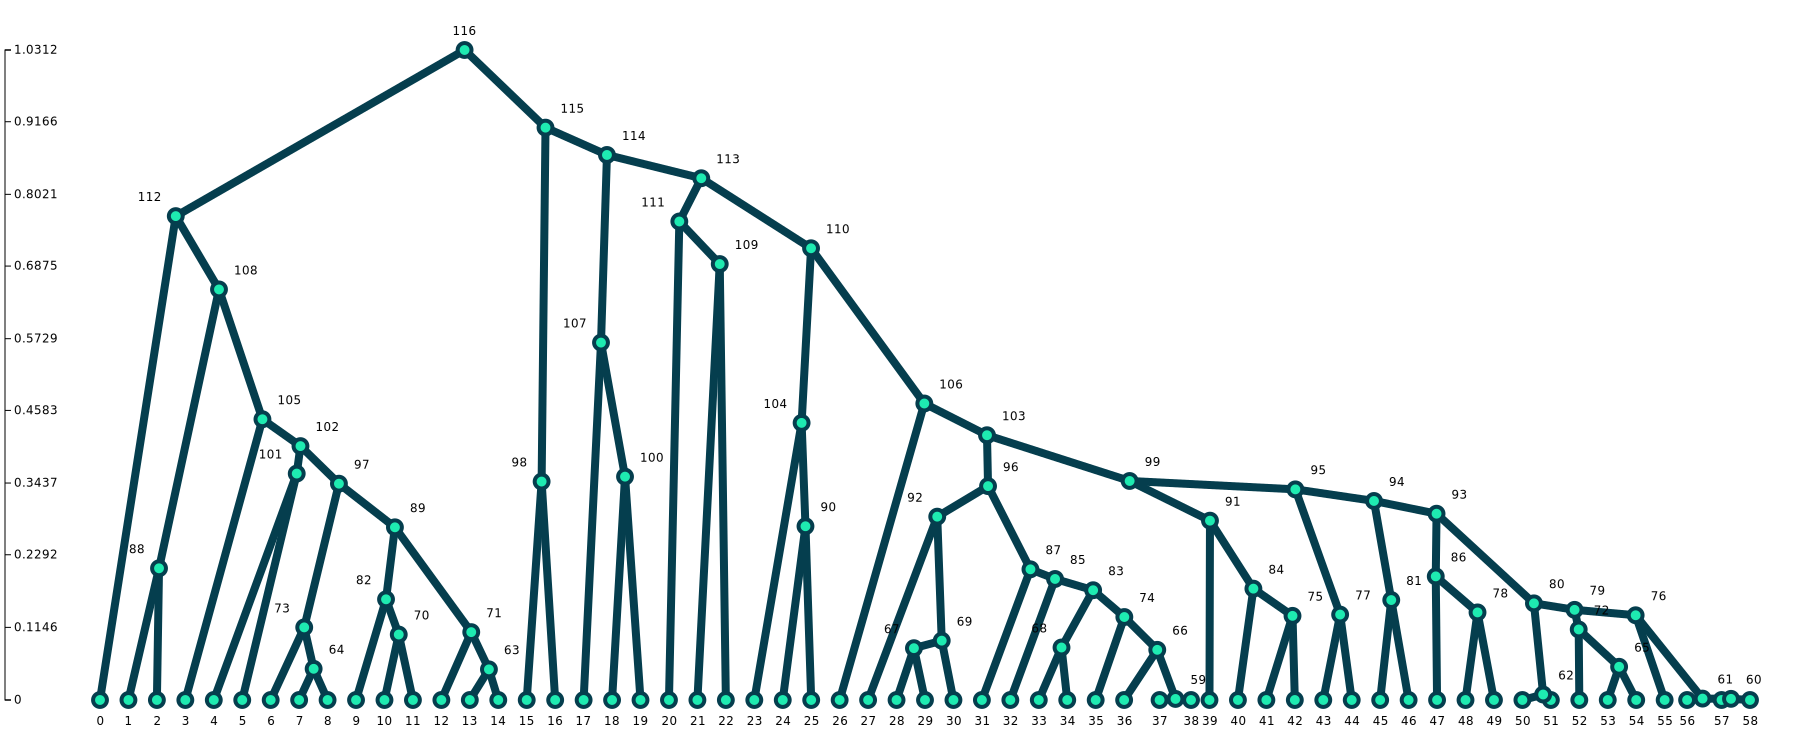
\includegraphics[width=0.49\textwidth]{figures/fitted_gfs/9.pdf}\\
    \caption[Fitted GFS for real-world pangenomes.]{True and simulated GFS for Bartonella quintana (top left), Staphylococcus argenteus (top right), Clostridium butyricum (bottom left), Buchnera aphidicola (bottom right).}
    \label{fig:fitted-gfs}
\end{figure}
With optimised parameters, our model successfully simulated matching GFS for most pangenomes but failed for some.
Although fitting is possible, as discussed in the previous section, it is slow due to the current Python-only implementation.
Therefore, we only used low sample count datasets.

Bartonella quintana, chosen due to its known high horizontal gene transfer rate \cite{Bartonella}.
Only 6 samples were present.
The fit is excellent, with a $\chi^2$ like error of 51 and an expected high resulting \ac{HGT} parameter of 0.003.
This would correspond to a rate of 30 if we rescale it by the number of sites.
As the used phylogenetic tree is balanced and the \ac{HGT} effect is strong, a characteristic \reflectbox{L} shape is visible.
An overview with all phylogenetic trees can be found in appendix \ref{app:panX-trees}.
\\
In addition, we selected another strain with slightly more samples where a high \ac{HGT} rate was expected.
We chose Staphylococcus argenteus as its part of the S. aureus related complex.
This strain had a similar \ac{HGT} value of 0.004
The fit is acceptable with a $\chi^2$ like error of 1170 and the significant right-shift of the \ac{GFS}
towards many high-frequency genes can be seen in the figure \ref{fig:fitted-gfs}.
It is important to note that the $\chi^2$ like error is not normalised and thus can't be compared directly between samples \ref{subsec:chi}.

In order to assess the model's capacity to handle the significant influence of the underlying phylogenetic tree,
we selected Clostridium butyricum, which exhibits a peak in the gene frequency class 9.
Despite the successful identification of parameters that resulted in matching \ac{GFS} for all other classes,
the optimisation algorithm was unable to identify parameters that replicated the peak in class 9.
This resulted in a $\chi^2$ line error of 749.
It is our hypothesis that the optimisation algorithm became trapped in local minima.
Local minima are particularly likely to occur when testing high gene conversion or \ac{HGT} rates.
The strong influence of these factors on the \ac{GFS}'s shape can significantly improve the $\chi^2$ like error in the first step,
but then also prevents the algorithm from identifying better parameters, as further changes to other parameters will have minimal impact.

As a representative example with a low rate of \ac{HGT} and a limited number of genes Buchnera aphidicola was chosen \cite{Buchnera}.
Unfortunately, due to its 59 samples, it resulted in a longer optimisation time, leading to unpolished parameters with a poor score. Here the fit resulted in a $\chi^2$ error of 701.
As the optimisation process had to be aborted due to the long run time and lack of computational resources, and as the results improved over time, we are optimistic that the fit could have been significantly better.

Differential Evolution proved to be significantly better than either \ac{SHGO} or
simple \ac{DS} for global optimisation. While \ac{DE} efficiently found reasonably good parameters for the first two samples in less than 1000 steps, \ac{SHGO} required over 2000 steps, leading to an impractically long runtime.

Therefore, after testing Bartonella quintana and Staphylococcus argenteus, we used \ac{DE} exclusively.
Locally, Downhill Simplex performs better than \ac{DE} and converges to a minimum faster.
Although \ac{DS} does not guarantee a global minimum, the variance of the local error is larger than the error itself, blocking any further minimisation.
This would be solved by using more simulations for each optimisation step to achieve a more stable $\chi^2$ like error, which would ultimately result in an impractical runtime.
